\documentclass[11pt]{article}
\usepackage[margin=1in]{geometry}
\usepackage{amsmath}
\usepackage{amssymb}
\usepackage{enumitem}
\usepackage{tikz}
\usepackage{multirow}
\usetikzlibrary{trees}

\title{Problem Set 4\\ECON 20100 -- Elements of Economic Analysis II}
\author{Kenneth C. Griffin Department of Economics, University of Chicago\\Winter 2026}
\date{Due: Wednesday, March 4, 2026}

\begin{document}

\maketitle

\noindent\textbf{Instructions.} Show all work. Clearly state any assumptions you make. Unsupported answers will not receive full credit. When asked to ``explain,'' a few precise sentences are expected.

\section*{Question 1: Monopoly Fundamentals [20 points]}

A monopolist faces inverse demand $P(Q) = 120 - 2Q$ and has total cost $C(Q) = Q^2 + 12Q$.

\begin{enumerate}[label=(\alph*)]
    \item \textbf{[4 points]} Derive the monopolist's marginal revenue function. Show that $MR < P$ for all $Q > 0$ and explain why in one sentence.
    \item[] $R=P\cdot Q=(120-2Q)\cdot Q=120Q-2Q^2\Rightarrow MR=\frac{\partial R}{\partial Q}=120-4Q<120-2Q=P$ for all $Q>0$. For monopolies, the marginal revenue of selling one more unit is less than the price because of the revenue lost on existing sales which requires that prices must fall.
    
    \item \textbf{[5 points]} Find the profit-maximizing quantity $Q^m$, price $P^m$, and profit $\pi^m$.
    \item[] $MC=\frac{\partial C}{\partial Q}=2Q+12$. Set $MR=MC\Rightarrow120-4Q=2Q+12\Rightarrow6Q=108\Rightarrow Q^m=18$. Then $P^m(Q^m)=120-2(18)=84$. Then $\pi^m=(Q^m\cdot P^m)-C(Q^m)=(18\cdot84)-(18^2+12(18))=1512-540=972$. So $(Q^m,P^m)=(84,18)$.
    
    \item \textbf{[5 points]} Find the competitive outcome $(Q^c, P^c)$ by setting $P = MC$. Compute consumer surplus, producer surplus, and total surplus under both monopoly and competition. What is the deadweight loss from monopoly?
    \item[] $P=MC\Rightarrow120-2Q=2Q+12\Rightarrow4Q=108\Rightarrow Q^c=27$. Then $P^c(Q^c)=120-2(27)=66$. So $(Q^c,P^c)=(27,66)$. Consumer surplus: $CS=\frac{1}{2}(P^{max}-P)(Q)$. Then $CS^m=\frac{1}{2}(120-18)(84)=324$, and $CS^c=\frac{1}{2}(120-66)(27)=729$. Producer Surplus: $PS=P\cdot Q-C$. Then $PS^m=(18\cdot 84)-((18^2+12(18))=1512-540=972=\pi^m$, and $PS^c=(66\cdot 27)-(27^2+12(27))=729=CS^c$. Total surplus: $TS=CS+PS$. Then $TS^m=324+972=1296$, and $TS^c=729+729=1458$. Deadweight loss: $DWL=TS^m-TS^c$. Then $DWL=1458-1296=162$.
    
    \item \textbf{[6 points]} Now suppose the monopolist's cost function changes to $C(Q) = 200 + 20Q$ (constant MC but with a fixed cost).
    \begin{enumerate}[label=(\roman*)]
        \item Find the new monopoly outcome $(Q^m, P^m, \pi^m)$.
        \item[] $MR$ same as above. $MC=\frac{\partial C}{\partial Q}=20$. Set $MR=MC\Rightarrow 120-4Q=20\Rightarrow 4Q=100\Rightarrow Q^m=25$. Then $P^m(Q^m)=120-2(25)=70$. Then $\pi^m=(Q^m\cdot P^m)-C(Q^m)=(25\cdot 70)-(200+20(25))=1750-700=1050$.
        \item Would a competitive market produce output in this case? \textit{Hint: What happens to a competitive firm with this cost structure?}
        \item[] $P=MC\Rightarrow 120-2Q=20\Rightarrow2Q=100\Rightarrow Q^c=50$. Then $P^c(Q^c)=120-2(50)=20$. Then $\pi^c=(Q^c\cdot P^c)-C(Q^c)=(50\cdot 20)-(200+20(50))=1000-1200=-200$. Thus, a competitive market would not produce output in this case because firms cannot cover fixed costs when $P=MC$, forcing them to leave the market and not produce.
        \item Explain how this example illustrates the concept of a natural monopoly, and discuss whether regulating this monopolist to set $P = MC$ would be sustainable.
        \item[] $AC=\frac{C(Q)}{Q}=\frac{(200+20Q)}{Q}=\frac{200}{Q}+20$. So $AC$ is decreasing in $Q$ and $AC>MC=20$ strictly for all $Q>0$. Thus, this is a natural monopoly because it is more efficient for one firm to produce for the entire market than for multiple firms to incur the fixed cost. Regulating this monopolist to set $P=MC$ is not sustainable as shown above because the firm would no longer cover its cost and would exit, leaving the market empty.
    \end{enumerate}
\end{enumerate}

\section*{Question 2: Price Discrimination [20 points]}

A monopolist sells in two segmented markets with inverse demands:
\[
P_1(Q_1) = 100 - Q_1, \quad P_2(Q_2) = 60 - Q_2
\]
The monopolist has constant marginal cost $MC = 20$ and no fixed costs. Assume the markets are completely separated (no arbitrage).

\begin{enumerate}[label=(\alph*)]
    \item \textbf{[5 points] Third-degree price discrimination.} Find the profit-maximizing price and quantity in each market. Which market gets the higher price? Relate your answer to the price elasticity of demand in each market at the optimal quantities.
    \item[] Market 1: $R=P_1\cdot Q_1=(100-Q_1)\cdot Q_1=100Q_1-Q_1^2\Rightarrow MR_1=\frac{\partial R}{\partial Q}=100-2Q_1\Rightarrow MR_1=MC\Rightarrow100-2Q_1=20\Rightarrow2Q_1=80\Rightarrow Q_1^*=40\Rightarrow P_1^*(40)=100-40=60$.
    \item[] Market 2: $R=P_2\cdot Q_2=(60-Q_2)\cdot Q_2=60Q_2-Q^2\Rightarrow MR_2=\frac{\partial R}{\partial Q}=60-2Q_2^2\Rightarrow MR_2=MC\Rightarrow60-2Q_2=20\Rightarrow 2Q_2=40\Rightarrow Q^*_2=20\Rightarrow P_2^*(20)=60-20=40.$
    \item[] Market 1 gets the higher price and thus has lower price-elasticity. Market 1 gets the lower price and thus has higher price elasticity. This is because a monopolist can charge higher prices without losing many sales when consumers are less price sensitive.
    
    \item \textbf{[4 points] Uniform pricing.} Suppose the monopolist is forced to charge a single price across both markets. Derive the aggregate demand curve (be careful---it has a kink). Find the optimal uniform price and total quantity.
    \item[] Deriving aggregate demand: Market 1: $Q_1=100-P_1$ when $P\leq 100$. Market 2: $Q_2=60-P_2$ when $P\leq 60$. There exists a kink at $P=60$. For $P\leq60$, $Q_t=Q_1+Q_2=(100-P)+(60-P)=160-2P\Rightarrow P(Q)=80-\frac{1}{2}Q_t$ if $Q>40$ (both markets active). For $60<P\leq100$, $Q_t=Q_1=100-P\Rightarrow P(Q)=100-Q_t$ if $Q\leq 40$ (only Market 1 active). 
    \item[] When both markets active: $TR=(80-\frac{1}{2}Q)\cdot Q=80Q-\frac{1}{2}Q^2   \Rightarrow MR=80-Q$. When Market 1 active: $TR=(100-Q)\cdot Q=100Q-Q^2\Rightarrow MR=100-2Q$. Set $MR=MC\Rightarrow 80-Q=20\Rightarrow Q^*=60>40$, checks so both markets active. Then $P^*=80-\frac{1}{2}(60)=50$. So $Q_t=Q_1+Q_2=(100-50)+(60-50)=50+10=60$.
    
    \item \textbf{[4 points]} Compare total output and total welfare $(CS + PS)$ under discrimination vs. uniform pricing. Does price discrimination increase or decrease total welfare here?
    \item[] Output under discrimination $=40+20=60=$ output under uniform pricing.
    \item[] Under discrimination: $CS_1=\frac{1}{2}(100-60)(40)=800$, $CS_2=\frac{1}{2}(60-40)(20)=200$, so $CS_t=800+200=1000$. $PS_t=(P_1^*-MC)(Q_1^*)-(P_2^*-MC)(Q_2^*)=(60-20)(40)+(40-20)(20)=1600+400=2000$. Then total welfare $=1000+2000=3000$.
    \item[] Under uniform pricing: $CS_1=\frac{1}{2}(100-50)(5)=1250$, $CS_2=\frac{1}{2}(60-50)(10)=50$, so $CS_t=1250+50=1300$. $PS_t=(P^*-MC)(Q_t)=(50-20)(60)=1800$. Then total welfare $=1300+1800=3100$. $3000<3100$, clearly price discrimination decreases total welfare here.
    
    \item \textbf{[7 points] First-degree price discrimination.} Now suppose the monopolist can perfectly identify each consumer's willingness to pay.
    \begin{enumerate}[label=(\roman*)]
        \item What quantity does the monopolist sell in each market? What is the monopolist's total profit?
        \item[] Set $P=MC$: $P_1=MC\Rightarrow100-Q_1=20\Rightarrow Q^*_1=80$, $P_2=MC\Rightarrow 60-Q_2=20\Rightarrow Q^*_2=40$. So $Q^*_t=80+40=120$. Profit: $\pi_1=\frac{1}{2}(100-20)(80)=3200$, $\pi_2=\frac{1}{2}(60-20)(40)=800$, so $\pi_t=3200+800=4000$. 
        \item What is consumer surplus? What is total surplus?
        \item[] Under perfect price discrimination, $CS=0$. Then total surplus $=PS=4000$.
        \item Is the outcome Pareto efficient? Explain how this is possible despite being a monopoly, and discuss why this outcome is unlikely in practice.
        \item[] This outcome is Pareto efficient because production occurs at $P=MC$ in both markets and there is no deadweight loss since the monopolist captures all gains from marginal quantity. This outcome is unlikely in practice because it is difficult for monopolists to know each consumer's exact willingness to pay, and to enact on this knowledge given logistics, consumer resistance. or legal constraints regarding price discrimination.
    \end{enumerate}
\end{enumerate}

\section*{Question 3: Second-Degree Price Discrimination [20 points]}

A software company sells to two types of consumers: ``professionals'' (type H) and ``students'' (type L). There are 100 consumers of each type. Their willingness to pay for two product versions are:

\begin{center}
\begin{tabular}{lcc}
\hline
 & Basic version & Premium version \\
\hline
Type H (professionals) & 40 & 100 \\
Type L (students) & 30 & 40 \\
\hline
\end{tabular}
\end{center}

The marginal cost of each version is zero. The firm cannot directly observe consumer types.

\begin{enumerate}[label=(\alph*)]
    \item \textbf{[4 points]} Suppose the firm only offers the Premium version. What is the profit-maximizing price, and what is the firm's profit?
    \item[] If $p_P=100$, only Type H buys. Profit $=100\times100=10000$. If $p_P=40$, both types buy. Profit $=40\times200=8000$. Since $10000>8000$, optimal price $p_P^*=100$, profit $\pi=10000$.
    
    \item \textbf{[4 points]} Suppose the firm offers both versions and can set separate prices $p_B$ (Basic) and $p_P$ (Premium). Write down the incentive compatibility (IC) constraint and the individual rationality (IR) constraint for each type.
    \item[] Individual Rationality: $IR_H: 100-p_P\geq0$ (Type H willing to buy Premium). $IR_L: 30-p_B\geq0$ (Type L willing to buy Basic). Incentive Compatibility: $IC_H: 100-p_P\geq40-p_B$ (Type H prefers Premium to Basic). $IC_L: 30-p_B\geq40-p_P$ (Type L prefers Basic to Premium).
    
    \item \textbf{[7 points]} Find the profit-maximizing prices $(p_B^*, p_P^*)$. Which constraints bind?\\
    \textit{Hint: The binding constraints are $IR_L$ (type L is just willing to buy Basic) and $IC_H$ (type H is just indifferent between Premium and Basic).}
    \item[] $\pi=100p_P+100p_B=100(p_P+p_B)$. Maximize $p_P+p_B$. Binding constraint $IR_L$: $30-p_B=0\Rightarrow p_B^*=30$. Binding constraint $IC_H$: $100-p_P=40-p_B\Rightarrow p_P=60+p_B=60+30=90$. So $(p_B^*,p_P^*)=(30,90)$. Check $IR_H$: $100-90=10\geq0$. Check $IC_L$: $30-30=0\geq40-90=-50$. So both constraints satisfied. Then $\pi^*=100(30)+100(90)=3000+9000=12000$.
    
    \item \textbf{[5 points]} Compare profits across the three regimes: (i) Premium only, (ii) menu pricing from part (c), and (iii) perfect price discrimination (the firm can observe types). Explain why the firm distorts the product line and what ``information rent'' type H earns.
    \item[] Premium only: $\pi=10000$. Menu pricing: $\pi=12000$. For perfect price discrimination: Charge Type H $p_P=100$, then profit from H $=100\times100=10000$. Also charge Type L $p_P=40$, then profit from L $=40\times100=4000$. Total profit $\pi=10000+4000=14000$.
    \item[] The firm distorts the product line by assigning Type L to Basic even though Type L values Premium more (40 vs 30) because offering Premium at low price would violate $IC_H$ and cause Type H to switch down. Information rent: Type H earns surplus $100-90=10$ per consumer, total rent $=10\times100=1000$. This occurs because the firm must price Premium low enough to prevent Type H from choosing Basic. The difference between perfect discrimination $(14000)$ and menu pricing $(12000)$ is $2000$, consisting of $1000$ information rent to Type H and $1000$ lost from inefficiently serving Type L with Basic instead of Premium at a higher price.
\end{enumerate}

\section*{Question 4: Strategic Interaction [20 points]}

\textbf{Part I.} Consider the following simultaneous-move game:

\begin{center}
\begin{tabular}{cc|c|c|c|}
 & \multicolumn{1}{c}{} & \multicolumn{3}{c}{Player 2}\\
 & \multicolumn{1}{c}{} & \multicolumn{1}{c}{L} & \multicolumn{1}{c}{C} & \multicolumn{1}{c}{R} \\\cline{3-5}
\multirow{3}*{Player 1} & U & $(3, 1)$ & $(0, 2)$ & $(1, 0)$ \\\cline{3-5}
 & M & $(1, 3)$ & $(2, 2)$ & $(3, 1)$ \\\cline{3-5}
 & D & $(0, 0)$ & $(1, 4)$ & $(2, 2)$ \\\cline{3-5}
\end{tabular}
\end{center}

\begin{enumerate}[label=(\alph*)]
    \item \textbf{[3 points]} Does either player have a strictly dominated strategy? If so, identify it and eliminate it.
        \item[] For Player 1: U vs M: $(3,0,1)$ vs $(1,2,3)$, has no dominance. U vs D: $(3,0,1)$ vs $(0,1,2)$, has no dominance. M vs D: $(1,2,3)$ vs $(0,1,2)$, M strictly dominates D since $1>0$, $2>1$, $3>2$. Thus Player 1 eliminates D. 
        \item[] For Player 2: L vs C: $(1,3,0)$ vs $(2,2,4)$, has no dominance. L vs R: $(1,3,0)$ vs $(0,1,2)$, has no dominance. C vs R: $(2,2,4)$ vs $(0,1,2)$, has no dominance. Thus there is no strictly dominated strategy for Player 2 and no strategy is eliminated.

    
    \item \textbf{[4 points]} After elimination, find all pure strategy Nash equilibria using the best response method. Show your work clearly.
    \item[] After eliminating D, reduced game:
    
\begin{center}
\begin{tabular}{cc|c|c|c|}
 & \multicolumn{1}{c}{} & \multicolumn{3}{c}{Player 2}\\
 & \multicolumn{1}{c}{} & \multicolumn{1}{c}{L} & \multicolumn{1}{c}{C} & \multicolumn{1}{c}{R} \\\cline{3-5}
\multirow{2}*{Player 1} & U & $(3, 1)$ & $(0, 2)$ & $(1, 0)$ \\\cline{3-5}
 & M & $(1, 3)$ & $(2, 2)$ & $(3, 1)$ \\\cline{3-5}
\end{tabular}
\end{center}
    
    \item[] P1 response: Given L, $3>1$, choose U. Given C, $2>0$, choose M. Given R, $3>1$, choose M. 
    \item[] P2 response: Given U, $2>1>0$, choose C. Given M, $3>2>1$, choose L. 
    \item[] Nash equilibria: Check (U,L): Player 1 plays U given L, but Player 2 deviates to C given U. Check (U,C): Player 1 deviates to M given C. Check (U,R): Player 1 deviates to M given R. Check (M,L): Player 1 plays M given L, and Player 2 plays L given M. So both are best responses. Check (M,C): Player 1 plays M given C, but Player 2 deviates to L given M. Check (M,R): Player 1 plays M given R, but Player 2 deviates to L given M. Then the only pure strategy Nash equilibrium is $(M,L)$ with payoffs $(1,3)$ for P1 and P2 respectively.
    
    
    \item \textbf{[3 points]} Are any outcomes in the original $3 \times 3$ game Pareto efficient? Identify all Pareto efficient outcomes and explain your reasoning.
        \item[] An outcome is Pareto efficient if no other outcome makes both players weakly better off with at least one strictly better off. The easiest way to check this is to observe the max payoffs for each player: P1 has a max payoff of 3 present in (U,L) and (M,R), P2 has a max payoff of 4 present in (D,C). At these positions, no move makes the maximum-benefiting weakly better off while also making the other strictly better off, thus they are Pareto efficient.

\end{enumerate}

\textbf{Part II.} Two firms simultaneously choose whether to invest in a new technology. The payoffs (in millions) are:

\begin{center}
\begin{tabular}{cc|c|c|}
 & \multicolumn{1}{c}{} & \multicolumn{2}{c}{Firm 2}\\
 & \multicolumn{1}{c}{} & \multicolumn{1}{c}{Invest} & \multicolumn{1}{c}{Don't} \\\cline{3-4}
\multirow{2}*{Firm 1} & Invest & $(4, 4)$ & $(-2, 6)$ \\\cline{3-4}
 & Don't & $(6, -2)$ & $(2, 2)$ \\\cline{3-4}
\end{tabular}
\end{center}

\begin{enumerate}[label=(\alph*)]
    \setcounter{enumi}{3}
    \item \textbf{[3 points]} Find all pure strategy Nash equilibria. Identify the game type (e.g., Prisoner's Dilemma, coordination game, chicken/hawk-dove).
    \item[] Firm 1 responses: Given Invest, $6>4$, choose Don't. Given Don't, $2>-2$, choose Don't. Firm 2 responses: Given Invest, $6>4$, choose Don't. Given Don't, $2>-2$, choose Don't. Nash equilibria: (Don't, Don't) since neither would deviate. This is a Prisoner's Dilemma game where players always prefer to Don't but would be better of if both chose to Invest.
    
    \item \textbf{[3 points]} Is the Nash equilibrium efficient? If not, explain intuitively why the firms fail to coordinate on a better outcome and propose one mechanism that might help.
    \item[] The Nash equilibrium with payoffs $(2,2)$ is not efficient. (Invest, Invest) with payoffs $(4,4)$ dominates the equilibrium since both firms would be strictly better off. Firms fail to coordinate because Don't is a dominant strategy for each firm: regardless of what the other firm does, each firm is individually better off choosing Don't. This creates a collective action problem where individual rationality leads to mutual harm. Once mechanism to help would be a binding agreement or regulation so that both can benefit without worry of deviation.

    
    \item \textbf{[4 points]} Now suppose the game is played sequentially: Firm 1 moves first, and Firm 2 observes Firm 1's choice before deciding. Draw the game tree. What is the subgame-perfect Nash equilibrium? Does sequential play help or hurt efficiency compared to simultaneous play?
    
\begin{center}
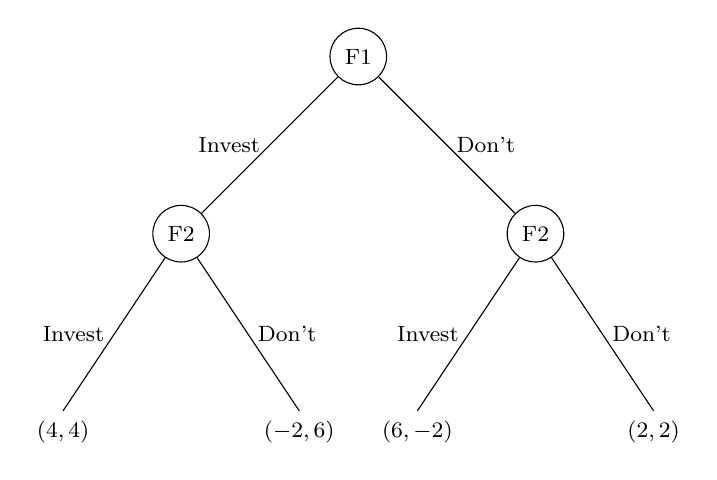
\begin{tikzpicture}[scale=1.5,font=\footnotesize]
  \node[circle,draw] (start) at (0,0) {F1};
  \node[circle,draw] (invest) at (-1.5,-1.5) {F2};
  \node[circle,draw] (dont) at (1.5,-1.5) {F2};
  
  \draw (start) -- node[left] {Invest} (invest);
  \draw (start) -- node[right] {Don't} (dont);
  
  \draw (invest) -- node[left] {Invest} (-2.5,-3) node[below] {$(4,4)$};
  \draw (invest) -- node[right] {Don't} (-0.5,-3) node[below] {$(-2,6)$};
  \draw (dont) -- node[left] {Invest} (0.5,-3) node[below] {$(6,-2)$};
  \draw (dont) -- node[right] {Don't} (2.5,-3) node[below] {$(2,2)$};
\end{tikzpicture}
\end{center}

\item[] Backward induction: At F2's decision node after F1 invests: $6>4$, choose Don't, payoff $(-2,6)$. At F2's decision node after F1 doesn't invest: $2>-2$, choose Don't, payoff $(2,2)$. At F1's initial node: If invest, get $-2$. If don't invest, get $2$. Since $2>-2$, F1 chooses Don't. Subgame-perfect Nash equilibrium: F2 plays Don't regardless of F1 and knowing this F2 also plays Don't. So sequential play does not help efficiency compared to simultaneous play.
\end{enumerate}

\section*{Question 5: Monopoly Meets Game Theory [20 points]}

An incumbent monopolist (firm I) earns monopoly profit $\pi^m = 100$ per period. A potential entrant (firm E) is deciding whether to enter the market. If E enters, the incumbent can either accommodate (share the market) or fight (engage in a price war). Payoffs per period are:

\begin{center}
\begin{tabular}{lcc}
\hline
Scenario & Incumbent & Entrant \\
\hline
E stays out & 100 & 0 \\
E enters, I accommodates & 40 & 30 \\
E enters, I fights & $-10$ & $-20$ \\
\hline
\end{tabular}
\end{center}

\begin{enumerate}[label=(\alph*)]
    \item \textbf{[4 points]} Write this as a sequential game (game tree) where E moves first (Enter or Stay Out) and I moves second (Accommodate or Fight, conditional on entry). Find the subgame-perfect Nash equilibrium using backward induction.
    
\begin{center}
\begin{tikzpicture}[scale=1.5,font=\footnotesize]
  \node[circle,draw] (start) at (0,0) {E};
  \node[circle,draw] (enter) at (-2,-1.5) {I};
  \node at (2,-1.5) {$(100,0)$};
  
  \draw (start) -- node[left] {Enter} (enter);
  \draw (start) -- node[right] {Stay Out} (2,-1.5);
  
  \draw (enter) -- node[left] {Accom.} (-3,-3) node[below] {$(40,30)$};
  \draw (enter) -- node[right] {Fight} (-1,-3) node[below] {$(-10,-20)$};
\end{tikzpicture}
\end{center}

\item[] Backward induction: At I's decision node $40>-10$, so I chooses Accommodate, giving payoffs $(40,30)$. At E's initial node $30>0$, so E chooses Enter. Subgame-perfect Nash equilibrium: I plays Accommodate after entry, and E plays Enter knowing this outcome leaving $(40,30)$.
    
    \item \textbf{[4 points]} Now write the game in normal (matrix) form, where E's strategies are \{Enter, Stay Out\} and I's strategies are \{Accommodate, Fight\}. Find all Nash equilibria of the normal form game. Identify any equilibrium that is not subgame-perfect and explain why.
    
\begin{center}
\begin{tabular}{cc|c|c|}
 & \multicolumn{1}{c}{} & \multicolumn{2}{c}{I}\\
 & \multicolumn{1}{c}{} & \multicolumn{1}{c}{Accommodate} & \multicolumn{1}{c}{Fight} \\\cline{3-4}
\multirow{2}*{E} & Enter & $(40, 30)$ & $(-10, -20)$ \\\cline{3-4}
 & Stay Out & $(100, 0)$ & $(100, 0)$ \\\cline{3-4}
\end{tabular}
\end{center}

\item[] E's responses: Given Accommodate, $30>0$ so choose Enter. Given Fight, $0>-20$, so choose Stay Out. I's responses: Given Enter, $40>-10$, so choose Accommodate. Given Stay Out, $100=100$, so indifferent between both actions. Two Nash equilibria: (Enter, Accommodate) and (Stay Out, Fight). However (Stay Out, Fight) is not subgame-perfect because in the subgame after Enter is reached, I would choose Accommodate $(40>-10)$. Fight is only rational on the path where E stays out and I is indifferent, but is irrational after entry.
    
    \item \textbf{[5 points]} The non-subgame-perfect equilibrium involves an ``incredible threat.'' Explain this concept. Why is the threat not credible even though it would benefit the incumbent if believed?
    \item[] An incredible threat is a commitment to take an action that would not be sequentially rational if actually called upon to execute it. In the equilibrium (Stay Out, Fight), I can threaten to Fight if E enters which deters E because of the negative payoff of $-10$ and then would preserve a monopoly profit of $100$ for I. However, the threat is not credible because if E actually entered, I's best sequential response in that subgame is to Accommodate $(40)$ rather than Fight $(-10)$, afraid of a negative payoff themselves. Since I would rationally deviate from Fighting if entry actually occurred, E should not believe the threat and should enter.
    
    \item \textbf{[7 points]} Now suppose the game is repeated infinitely, with both firms using discount factor $\delta \in (0, 1)$.
    \begin{enumerate}[label=(\roman*)]
        \item Suppose I announces the following strategy: ``I will fight any entrant, forever.'' If E believes this, what is E's expected payoff from entering? For what values of $\delta$ would E choose to stay out?
        \item[] If I fights forever after entry, then E receives payoff of $-20$ in every period after entering. Present value: $PV_E=-20+\delta(-20)+\delta^2(-20)+\cdots=-20\sum_{t=0}^{\infty}\delta^t=-20\cdot\frac{1}{1-\delta}=\frac{-20}{1-\delta}<0$ for all $\delta\in(0,1)$. But if E stays out, E receives $0$ in every period, giving a  $PV_E=0$. Since $0>\frac{-20}{1-\delta}$ for all $\delta\in(0,1)$, E chooses to stay out for all values of $\delta\in(0,1)$.
        \item Now suppose there are $T$ potential entrants who arrive sequentially (one per period). Can the incumbent use a ``fight always'' strategy to deter all entrants? For what values of $\delta$ does this work?
        \item[] If I fights all entrants, I receives $-10$ per period during fights (periods $1$ through $T$), then monopoly profit $100$ forever after. If I accommodates the first entrant, I receives $40$ per period forever. Present value of fighting all $T$ entrants: $PV_{fight}=\sum_{t=1}^{T}(-10)\delta^{t-1}+\sum_{t=T+1}^{\infty}100\delta^{t-1}=-10\cdot\frac{1-\delta^T}{1-\delta}+100\delta^T\cdot\frac{1}{1-\delta}=\frac{-10+110\delta^T}{1-\delta}$. Present value of accommodating first entrant: $PV_{accom}=\sum_{t=1}^{\infty}40\delta^{t-1}=\frac{40}{1-\delta}$. I prefers to fight all if $\frac{-10+110\delta^T}{1-\delta}\geq\frac{40}{1-\delta}$, which gives $-10+110\delta^T\geq40$, so $110\delta^T\geq50$, thus $\delta^T\geq\frac{5}{11}$. This requires $\delta\geq\left(\frac{5}{11}\right)^{1/T}$. For $\delta\geq\left(\frac{5}{11}\right)^{1/T}$, the fight always strategy can deter all $T$ entrants.
        \item Does the ``fight always'' strategy survive backward induction when $T$ is finite? Explain the unraveling argument. How does this change when $T = \infty$?
        \item[] When $T$ is finite, the fight always strategy does not survive backward induction due to unraveling. In period $T$, the last potential entrant knows there are no future entrants for I to deter. At this final decision, since $40>-10$, I will accommodate entrant $T$. But knowing this themselves, entrant $T$ will enter. And in period $T-1$, I also knows that entrant $T$ will enter regardless of what happens in period $T-1$. Therefore, fighting entrant $T-1$ provides no future benefit to reputation building. So I continues to choose Accommodate. This logic unravels backward to period $1$: I accommodates the first entrant because the finite $T$ eliminates any reputational benefit from fighting. However, when $T=\infty$, there is no final period where backward induction can begin. The threat to fight forever can then be sustained if $\delta$ is sufficiently high. At any period, I's decision to fight preserves the reputation that deters all future infinite entrants, making the short-term costs of fighting $(-10$ vs $40)$ worthwhile for the longer-term benefit of monopoly profit $(100)$ forever after this reputation has been established.
    \end{enumerate}
\end{enumerate}

\vspace{1cm}
\begin{center}
\textit{End of Problem Set 4}
\end{center}

\end{document}